% Thesis introduction
% Author: Tore.
%

In this chapter the background information needed in order to understand the topics of this thesis and its papers is given. First, in Section \ref{sec:gpgpu}, general-purpose computing on graphics processing units (\nom{GPGPU}{General-purpose computing on graphics processing units}) is reviewed, followed by an introduction to medical ultrasound imaging in Section \ref{sec:ultrasound}. Finally, the concepts of volume rendering and ultrasound field simulations are presented in Section \ref{sec:volren} and \ref{sec:field}.

\section{General-purpose computing on graphics processing units}\label{sec:gpgpu}
In a recent essay, Herb Sutter, a leading authority on software development, reviews the current state of the software and computer industry \cite{HerbSutter}. The essay bears the name "Welcome to the Jungle" and is a sequel to the essay "The Free Lunch is Over" from 2004 \cite{HerbSuttera}. The two essays spins around the fact that manufactures of central processing units (CPU) hit a frequency-wall in the beginning of the 21st century. Until then, all mainstream computer programs where typically running in a single thread on a single CPU \textit{processing core}, and a programmer could expect the software to annually gain performance without touching the code. This was the "free-lunch"-era as depicted in Fig.\,\ref{fig:jungle}. The increase in processing power came mostly from an ever-growing clock frequency. However, power consumption and heat generation where also growing at the same rate, until the level of cooling required finally became to much in 2004.  From that point, chip manufactures had to pursue a different direction  than just increasing the clock frequency. The immediate solution was to embed several cores in one CPU. This insured continuation of Moore's law, since the number of transistors per chip could continue to grow. For programmers, multi-core CPUs meant that computer programs now had to be multi-threaded in order to annually gain performance. It was a concurrency revolution, as Herb Sutter named it, and  the "free lunch" was over.

\begin{figure}
\centering
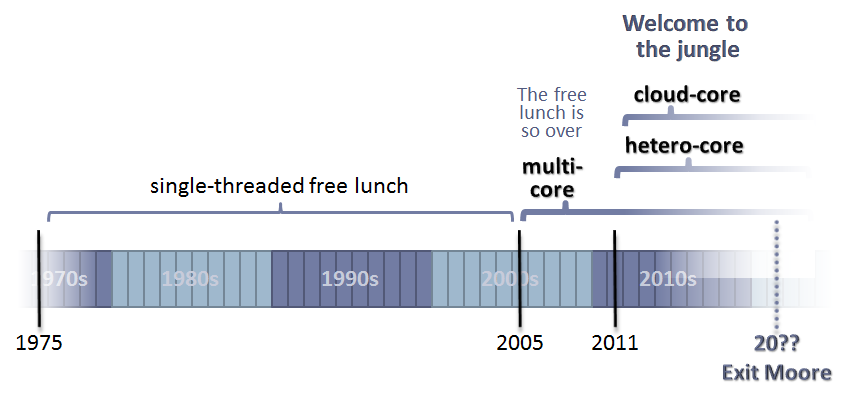
\includegraphics[width=0.8\textwidth]{img/free_lunsh.png}
\caption{Illustration of transitions between different eras in the computer industry. Currently there are three ongoing transitions; multi-core, heterogeneous-core and cloud-core. Image courtesy of Herb Sutter (herbsutter.com).}
\label{fig:jungle}
\end{figure}

Around the same time as CPU manufactures hit the frequency wall, people started experimenting with programmable shaders which recently had been introduced in the field of graphics programming. The graphics processing pipeline had before this been a fixed function pipeline, where e.g. geometry and textures where fed to the graphics processing unit (GPU) in one end, and where shaded a rasterized geometry was outputted in the other. What programmable shaders  introduced was the ability to replace some steps in the fixed-function pipeline with custom computations. This made it possible to utilize the GPU for other tasks than just rendering graphics \cite{Seland2007}. The rationale behind this exploration was that GPUs were already highly available in consumer PCs, and hidden behind its graphics interface were processing powers an order of magnitude larger than what the CPU could provide (Fig.\,\ref{fig:cpu_vs_gpu}). Actually, at the time when CPU manufacturers hit the frequency wall the GPU had already gone multi-core, first of all driven by an ever-increasing demand for more realistic computer games. Second, the rendering pipeline exhibits minimal execution path branching, and data are typically used once. Designers of GPUs could therefore skip advance feature, found in most CPUs, like branch prediction and different levels of data caching. These measures reduced the silicon footprint of each core and made it possible to add multiple cores to one GPU before CPU designers where able to do the same. Today, even if more advanced caching has been added to GPUs, this is still the main reason why GPUs have higher peak performance than CPUs (Fig.\,\ref{fig:cpu_vs_gpu}). Another reason is the inherent parallel nature of the rendering problem. When geometry is shaded, projected and rasterized the same instruction is typically needed for a lot of data at the same time. This makes a special kind of instruction, known as Single Instruction Multiple Data (\nom{SIMD}{Single instruction multiple data (instruction)}) \cite{Flynn1966}, especially suited for this kind of problem. The differences between how SIMD instructions are utilized in modern CPUs and GPUs are discussed in Section \ref{sec:cpu_vs_gpu}.

For the first adopters general-purpose computing on GPUs (GPGPU) it soon became evident that offloading all types of computations to the GPU was not always a good idea. In most cases it is important to balance the load equally between the CPU and GPU to obtain their combined computationally power. Balancing typically means that highly parallel and computationally intense tasks should be offloaded to the GPU and serialized and memory intensive work should stay on the CPU. This paradigm of utilizing specialized cores for solving specific problems is today known as heterogeneous computing. The specialized core can be a GPU or e.g. a field-programmable gate array (\nom{FPGA}{Field-programmable gate array}). A recent trend is that specialized accelerator cores are embedded onto the CPU. This heterogeneous processors is often referred to as an accelerated processing unit (\nom{APU}{Accelerated processing unit}). The last three generations of CPUs from Intel have all had on-chip integrated graphics. Even if an on-chip GPU is less powerful than a high-performance discrete GPU, valuable time is saved by not having to send data across the PCI Express bus, which connects the different parts of a computer to the motherboard. This is the reason why one of the first rules of GPGPU (with discrete GPUs) is to minimize CPU-to-GPU memory transfers. 

The final transition currently taking place in the computer industry is the introduction of cloud computing, where compute power is provided as a web-service and automatically scales on demand. Together, multi-core, heterogeneous cores, and cloud cores forms the "jungle" that today's software engineers have to tackle (Fig.\,\ref{fig:jungle}). In this thesis we focus on heterogeneous computing with one multi-core CPU and a discrete high performance GPU, a cheap and high performance system which is likely to be the specification of current and future ultrasound imaging system.

\subsection{Comparing CPU and GPU performance}\label{sec:cpu_vs_gpu}
The CPU is design to be the main control unit of a computer. It is therefore good at general processing. The GPU, on the other hand, has a history of processing graphics which involves heavy vector arithmetic. Even though they started out as very different processors, modern CPUs are including more and more GPU-like features, and GPUs are adding CPU features. In this section we will see what these similarities are and why there is still a big difference in peak performance between a CPU and a GPU.

\begin{figure}
\centering
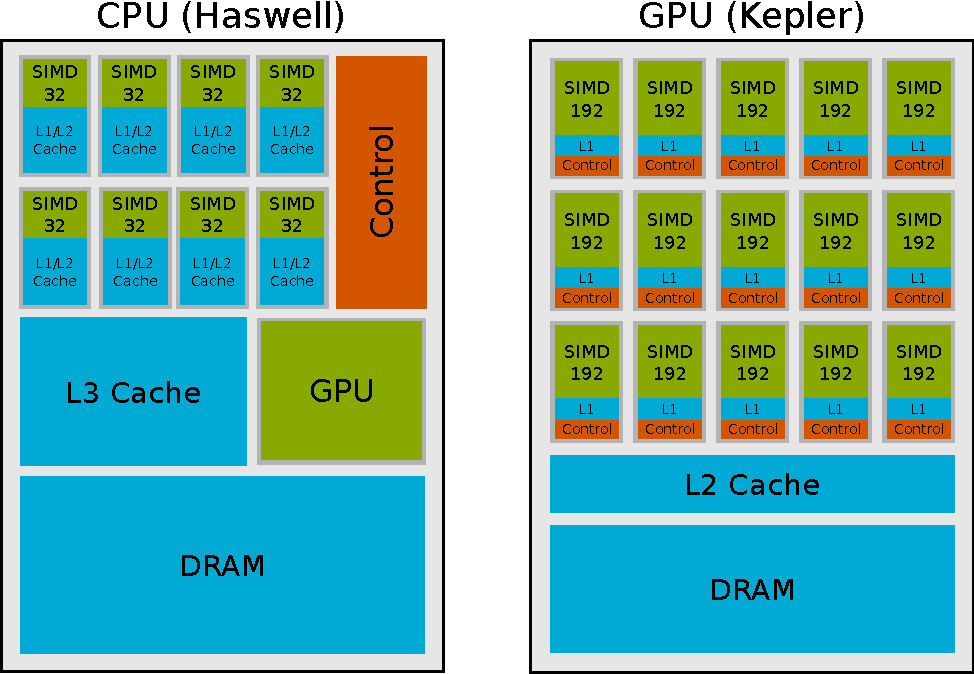
\includegraphics[width=0.8\textwidth]{img/CPU-GPU.pdf}
\caption{Schematic overview of CPU (Intel Haswell) and GPU (Nvidia Kepler) architecture. Note how more space is dedicated to compute cores on a GPU, and how more space is dedicated to control and caching on a CPU.}
\label{fig:cpu_gpu}
\end{figure}

In Section \ref{sec:gpgpu} we introduced a special type of instructions, namely SIMD instructions, which are designed to execute a single instruction across multiple data element in one clock cycle. At the end of the 20th century, Intel introduced a SIMD instruction set for their Pentium III processor called the Streaming SIMD Extensions (\nom{SSE}{Streaming SIMD extensions (instruction)}). This extension has seen several updates since. The first SEE instructions set had 128 bit long registers which meant that four, 32 bit, floating point values could be processed per clock cycle\footnote{For simplicity we will assume that the whole register is processed in one clock cycle even if the actual implementation might distributes one instruction for the register across multiple cycles.}. Updates of the SSE instruction set have added new instructions (SSE2, SSE3, and SSE4) and longer registers (\nom{AVX}{Advanced vector extensions (instruction)}, AVX2, and AVX-512). AVX and AVX2 adds 256 bit long registers and fused multiply-accumulate instructions (\nom{FMA}{Fused multiply-accumulate (instruction)})  which means that sixteen 32 bit floating point values can be processed per clock cycle per core. A new extension, AVX-512, extends the registers to 512 bit and is found in the Intel accelerator board  Xeon Phi and might show up in the next generation of CPUs from Intel. The latest CPU architecture from Intel, the Haswell architecture, has two processing ports supporting FMA-AVX2 instructions, and is therefore capable of processing 32, 32 bit, floating point values per clock cycle per core (Fig.\,\ref{fig:cpu_gpu}). For an eight core\footnote{An 8-core Haswell CPU is scheduled to launch during 2014.} CPU with a clock frequency of 3.8 GHz this sums to 
\begin{equation}
32*8*3.8 = 972.8\,\text{GFLOPS},
\end{equation}
hence a theoretical peak performance of close to one tera single precision floating point operations per second (TFLOPS). This is the same number as visualized in Fig\,\ref{fig:cpu_vs_gpu} for the Haswell architecture. In addition, the most powerful integrated GPU found on Haswell CPUs (HD 5200) have 40 execution units capable of processing sixteen, 32 bit, floating points at 1.3 GHz. This adds
\begin{equation}
16*40*1.3 = 832\,\text{GFLOPS}
\end{equation}
in extra processing power to the APU.

Modern GPUs can also be interpreted as a unit consisting of multiple SIMD processors (Fig.\,\ref{fig:cpu_gpu}). The Kepler architecture by Nvidia have up to 15 SIMD units capable of processing 192, 32 bit, floats per clock cycle at 745 MHz. These GPUs are also capable of performing FMA instructions, effectively doubling the number of theoretical FLOPS. The theoretical peak single precision FLOPS for this architecture is by that found to be 
\begin{equation}
15*192*2*745 = 4291\,\text{GFLOPS}.
\end{equation} 
Each SIMD core also comprise 16 special function units (\nom{SFU}{Special function unit (sin, exp, sqrt, ect.)}) which add close to 1 TFLOPS in additional computational power. This adds up to a total of five TFLOPS in computationally power as shown in Fig.\,\ref{fig:cpu_vs_gpu} for the GeForce GTX 780 TI GPU. From Fig.\,\ref{fig:cpu_gpu} we see how the high number of SIMD cores found on GPUs and their larger width, compared with SIMD cores on the CPU, results in five times the computational performance of a high-end CPU (without the integrated GPU). 

Note that the derived numbers are strictly theoretical and that actual throughput is highly algorithm dependent. Nevertheless, in theory, the benefit of GPU computing over CPU computing is currently a factor of five in raw computationally power. A claimed speed-up of several order of magnitude is typically caused by comparing a non-optimized CPU implementation with an optimized GPU implementation or by comparing uneven hardware \cite{Lee2010, Kothapalli2013}. Also note that in this section we have focused on CPUs from Intel and GPUs from Nvidia, however, CPUs and GPUs from AMD have similar specifications. 

\begin{figure}
\centering
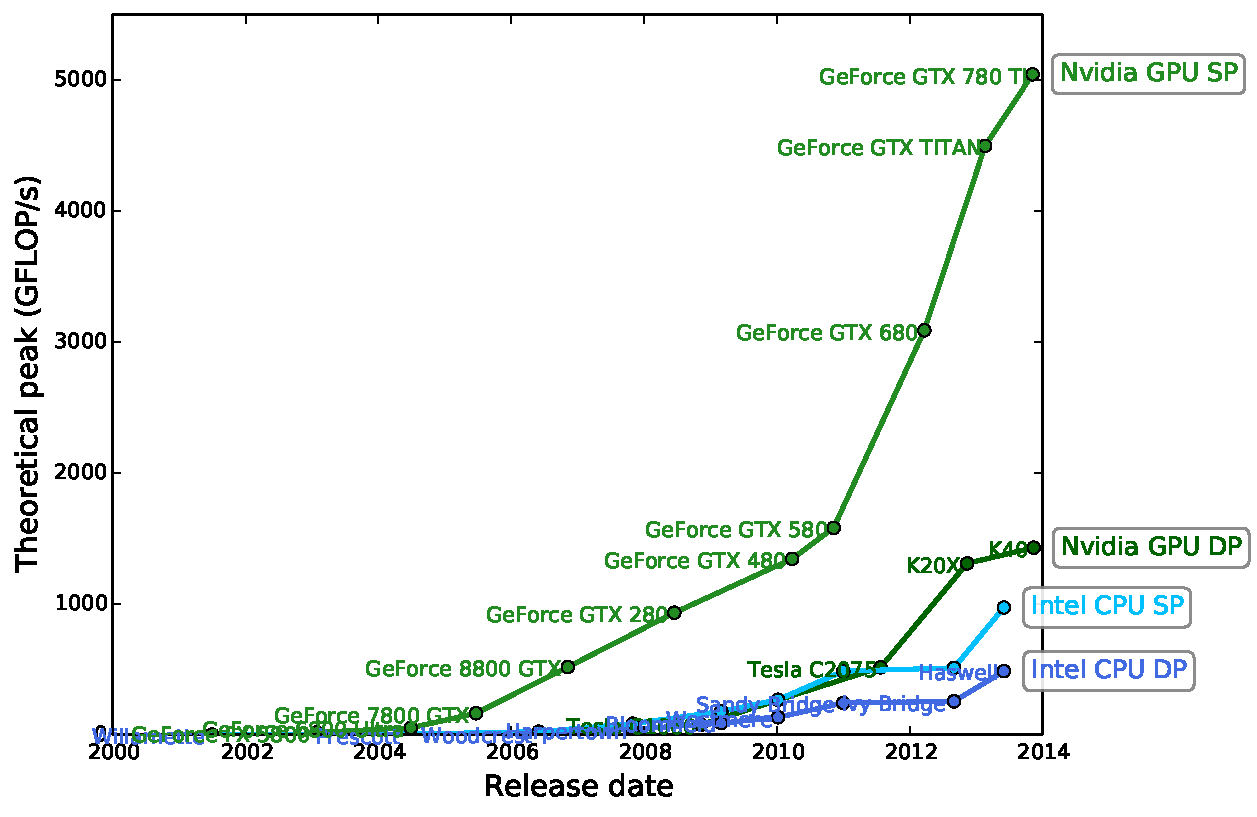
\includegraphics[width=\textwidth]{img/cpu_vs_gpu.pdf}
\caption{Development in theoretical peak throughput, single precision (SP) and double precision (DP), the last decade for Intel CPUs and Nvidia GPUs.}
\label{fig:cpu_vs_gpu}
\end{figure}

\subsection{Programming a GPU}
Early GPGPU programming required expert knowledge about computer graphics and the remaining fixed functions in the pipeline. When GPGPU gained interest it quickly became evident that new programing languages where needed.  One of the first GPGPU oriented languages for the GPU was the Brook language by Buck \textit{et al.} \cite{Buck2004}. Buck later joined Nvidia where he led the work on \nom{CUDA}{Compute unified device architecture (GPGPU language)}, a GPGPU language and framework by Nvidia for Nvidia GPUs only. The first version of CUDA was released in 2007. The following year, Apple launched a GPGPU framework known as \nom{OpenCL}{Open Compute Language (GPGPU language)}, a standard which are maintained by the Khronos Group. These two frameworks are still today the main programming frameworks for GPGPU. Where CUDA only runs on Nvidia GPUs, OpenCL can now run on GPUs from both Nvidia and AMD, CPUs from both Intel and AMD, FPGAs from Altera, and mobile processors from \nom{ARM}{Designer of mobile chip architectures}.

\begin{figure}
\centering
\subfigure[Kernel]{
	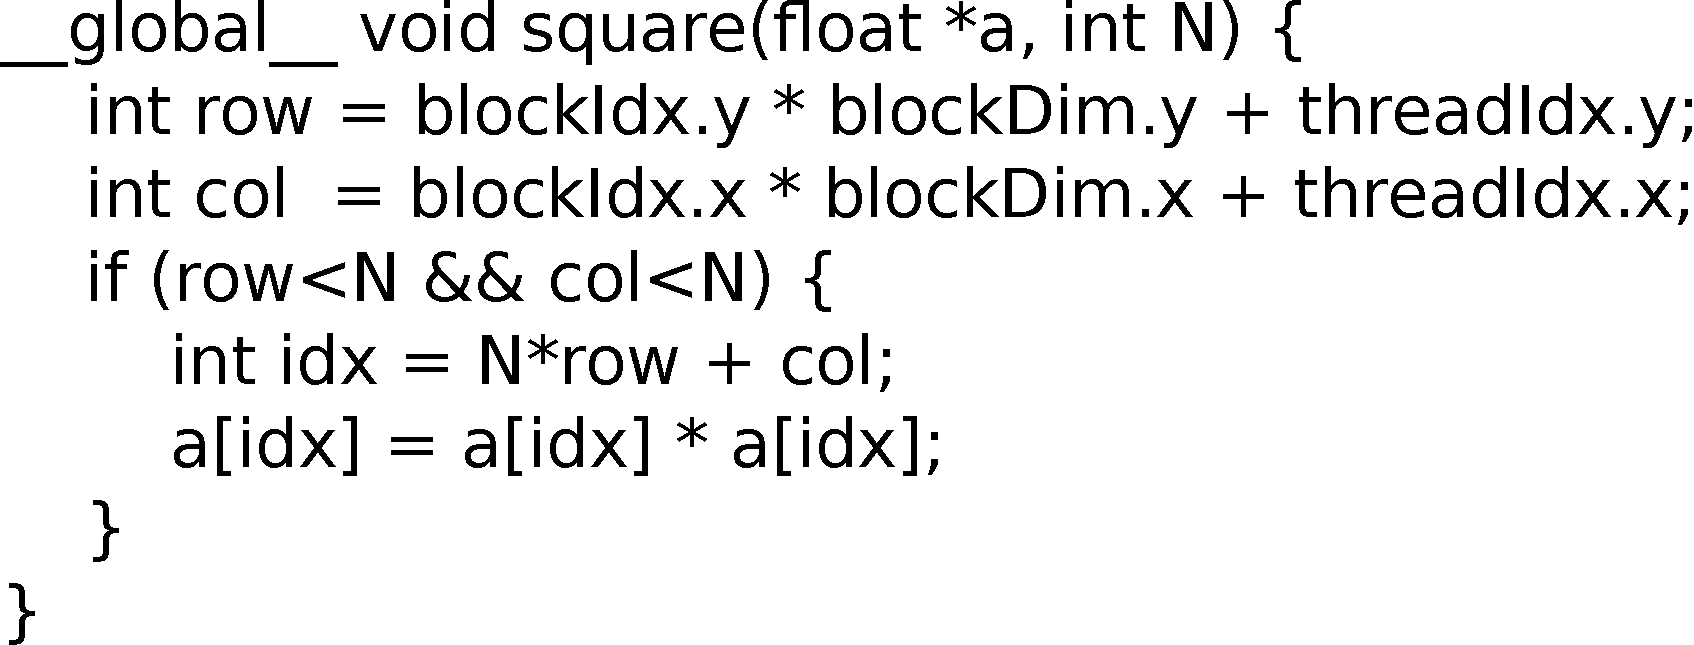
\includegraphics[width=0.5\textwidth]{img/kernel.pdf}\label{fig:gpu_kernel}
}
\subfigure[Threads, blocks and grid]{
	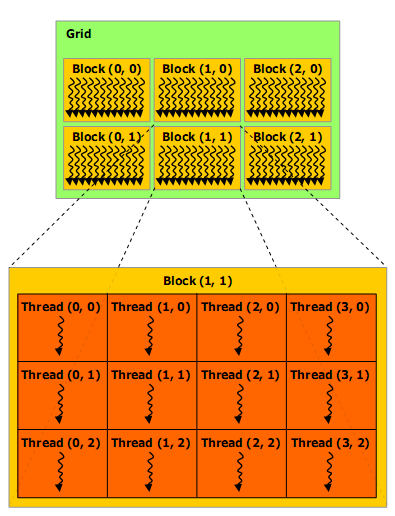
\includegraphics[width=0.4\textwidth]{img/cuda_threads.png}\label{fig:gpu_grid}
}
\caption{The figure depicts how GPU threads are grouped into blocks and arranged in a grid. One thread runs a copy of a kernel function. In this example the kernel function performs an element-wise matrix square.}
\label{fig:gpu_grid_kernel}
\end{figure}

Both CUDA and OpenCL is centered around a kernel function which are executed by a large group of threads. The kernel function, for both CUDA and OpenCL, has a C-like syntax with some additional specifiers. A CUDA kernel is depicted in Fig.\,\ref{fig:gpu_kernel}. The \texttt{\_\_global\_\_} specifier tells the CUDA compiler that this function is a kernel function, and in CUDA, this kernel function is launched by using a CUDA specific syntax:
\begin{align*}
\texttt{square<<<grid, block>>>(a, N)},
\end{align*}
where \texttt{grid} and \texttt{block} is 3-component vectors specifying grid and block size in "xyz" as depicted in Fig.\,\ref{fig:gpu_grid}, \texttt{a} is a pointer to a memory buffer located on the GPU, and \texttt{N}$*$\texttt{N} is the buffer size. When launched, a copy of the kernel is scheduled  for each thread in each block, and each kernel get as input its location in the compute grid (\texttt{blockIdx} and \texttt{threadIdx}) together with the grid size (\texttt{gridDim} and \texttt{blockDim}). This information is then typically used to calculate which memory elements to gather from the global memory buffer \texttt{a}. In order to formulate a given problem as a kernel function the global memory input to each thread must not rely on the output from other threads, hence it must be possible for the GPU to scheduled threads in any order. 

This is of course a minimal example of GPU programing. A full example will involve several lines of code transferring data to and from the GPU, and the kernel could include manual administration of the L1 cache (shared memory), and intra-block thread barriers. This is some of the reasons why writing a high performance GPU kernel is too often found to be a complex and time consuming task. 

No doubt, it is still a major overhead involved with writing GPU code, and in the future we will probably see work aimed at reducing this overhead.  A recent development is the introduction of C++ AMP which enables developers to write accelerated code (e.g. by a GPU) in plain C++. Hopefully, in the future, GPU programming will be a job for compilers, and direct fiddling with GPU kernels should only be needed if maximum throughput is absolutely needed. This is similar to how SIMD instructions is handled in CPU code today. Most of the time developers will rely on the CPU compilers to analyze the code and auto-apply SIMD instruction whenever it is possible. However, when maximum throughput is needed, developers with deep knowledge of the problem at hand are often able to make faster code by manually writing SIMD instruction code. The relevance of auto-applied GPU instructions by compilers will also increasing due to the recent embedding of GPUs on the same chip as the CPU. Soon, when writing code, we will probably talk about coding for a collection of heterogeneous cores where operations are automatically offloaded to special cores (e.g. a GPU) by the compiler.

\section {Medical ultrasound imaging}\label{sec:ultrasound}
Ultrasound imaging encompasses technology which generates images based on sound whose frequencies we can not hear. For medical ultrasound imaging frequencies between 2 MHz and 10 MHz are typically used. Frequency dependent attenuation force us to select a lower frequency if the object we want to image is located deep into the body. This is the reason why 2-4 MHz is used for cardiac imaging and a frequency around 7 MHz is used for vascular imaging. A piezoelectric ceramic is used to generate the ultrasonic frequencies, and is special in that way that ultrasound vibrations are generated when voltage is applied and \textit{vice versa}. It can therefore be used to both send and receive ultrasound signals, like a combined microphone and speaker. Piezoelectric elements organized in an array, is referred to as an ultrasound \textit{probe}, and a special probe is typically design for each medical imaging modality. For cardiac ultrasound imaging the probe footprint has to be smaller than the intercostal window in order to avoid shadowing by ribs. A line in an ultrasound image is generated by firing a ultrasound pulse into the body and sample the received echo. This amplitude trace is known as an A-mode image.    

If the width of a piezoelectric element is less than the wavelength of the transmitted signal the element is said to be \textit{omnidirectional}, hence energy is distributed equally in all directions. When multiple omnidirectional elements are arranged in an array the transmitted pulse will get shaped into a beam\footnote{A beam refers to the pulse integrated in time.} of ultrasound by diffraction. The 3 dB angular width of this beam, and also the angular resolution of the array, is given by \cite{AngelUltrasound}:
\begin{align}
\delta\theta = \frac{\lambda}{D},
\end{align}
\nomi{$\delta\theta$}{Angular resolution} where \nom{$\lambda$}{Wavelength} is the ultrasound wavelength, and \nom{$D$}{Aperture width} is the aperture width. With a speed-of-sound in human tissue of $1540\frac{\text{m}}{\text{s}}$ the angular resolution of a 2 cm cardiac array at 3 MHz is around 1.5\degree, which at 8 cm gives a lateral resolution of 2 mm. The axial resolution is inverse proportional to the pulse length, and is typically better than the lateral resolution.

If time delays are applied on the signal sent to the different elements it is possible to steer and focus the ultrasound beam in space. This technique is know as \textit{beamforming}, and for ultrasound imaging it is applied both when transmitting and receiving ultrasound pulses. For medical ultrasound imaging there are two main types of ultrasound probes, linear and phased arrays \cite{AngelUltrasound}. A cardiac ultrasound array is a phased array, which means that the image is constructed from beams, or A-mode images, which are gradually steered from $-\theta/2$ to $\theta/2$, resulting in sector which are $\theta$ wide. This kind of image is known as a B-mode image (B for brightness). If \nom{$M$}{Number of array elements} is the number of elements in the array, and \nom{$\Delta_m[n]$}{Per-element focusing and steering delays} is the per-element focusing and steering delay, the beamforming technique known as \textit{delay-and-sum} is given as:
\begin{align}\label{eq:das}
z[n] = \sum_{m = 0}^{M-1}\vec{w}_m^*\vec{x}_m[n - \Delta_m[n]] = \vec{w}^H\vec{x}[n],
\end{align}
where \nom{$\vec{w}$}{Array weight vector (apodization)} is know as the array weight vector or apodization, and $z[n]$ is an A-mode image.  If the phase center of our array is the origin and $p$ is the point where we want to steer and focus the ultrasound beam we have to use delays given as:
\begin{align}
\Delta_m[n] =\frac{|x_m+p| - |p|}{c},
\end{align}
where $c$ is the speed of sound.

%The weight vector is typically selected in order to trade resolution for a lower side lobe level. Hence, the weights are typically real and their K-space response is then symmetric.

Typical probes, scan sequences, resolution and sampling.

Sampling rates, and data size.

Delay and sum. Apodization. (See intro to Paper II or III).
Time v.s. phase delays.

Key selling points of ultrasound imaging: cost, safety and real-time user interaction.

One sentence about speckle tracking.

\begin{figure}
\centering
\subfigure{
	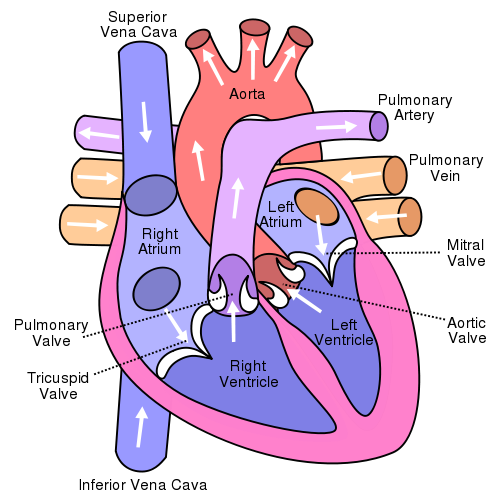
\includegraphics[width=0.47\textwidth]{img/Diagram_of_the_human_heart.png}
}
\subfigure{
	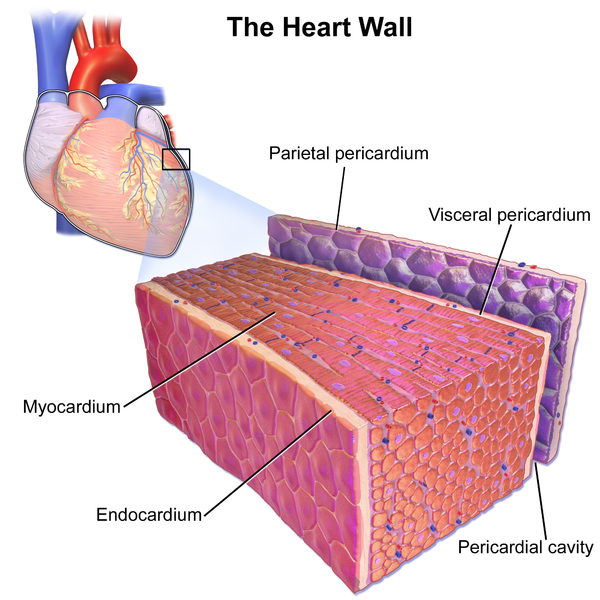
\includegraphics[width=0.47\textwidth]{img/HeartWall.png}
}
\caption{Overview of the human heart. Illustrations from wikipedia.org.}
\label{fig:human_heart}
\end{figure}

Small section about heart anatomy.

\subsection{Accelerators in medical ultrasound imaging}
Ultrasound imaging systems generates an incredible amount of data. A modern system capable of 3D imaging will generate several tera bytes of data in the front end of the system during a clinical scan. The data rate from a 2D scan is "only" in order giga bytes per second. To handle these amount of data, ultrasound imaging systems have relied heavily on application-specific integrated circuits (\nom{ASIC}{Application-specific integrated circuit}) for all steps in the processing pipeline. However, as the computationally power of CPUs and GPUs have increased, ASICs, e.g. for scan conversion, have gradually been converted into software \cite{Guracar2013}. One of  the last remaining ASICs is the beamformer, whose job is to steer and focus the ultrasound beam in space. This operation involves a reduction of the data rate with a factor equal to the number of elements in the ultrasound probe. The input data rate is therefor very high. Nevertheless, real-time beamforming has recently been achieved on a GPU \cite{Song2012}, and a French company (SuperSonic Imagine) are utilizing GPUs in their plane wave ultrasound beamforming algorithm \cite{Tanter2014}. Beamforming is therefore finally moving into software to. The largest players in the medical ultrasound business, General Electric and Philips, are also well aware of where the trend is going \cite{Thomenius2012} \cite{Metz2011}. Software beamforming opens up new possibilities for advanced processing. One example is Capon beamforming which is explored in this thesis (\textbf{Paper\,I} and \textbf{II}), another is advanced 3D visualization as presented in \cite{solteszova2010multidirectional}, \textbf{Paper\,IV}, and \textbf{IX}.

\subsection{Adaptive Beamforming}\label{sec:adaptbf}

\begin{figure}[t!]
\subfigure[Delay-and-sum]{
	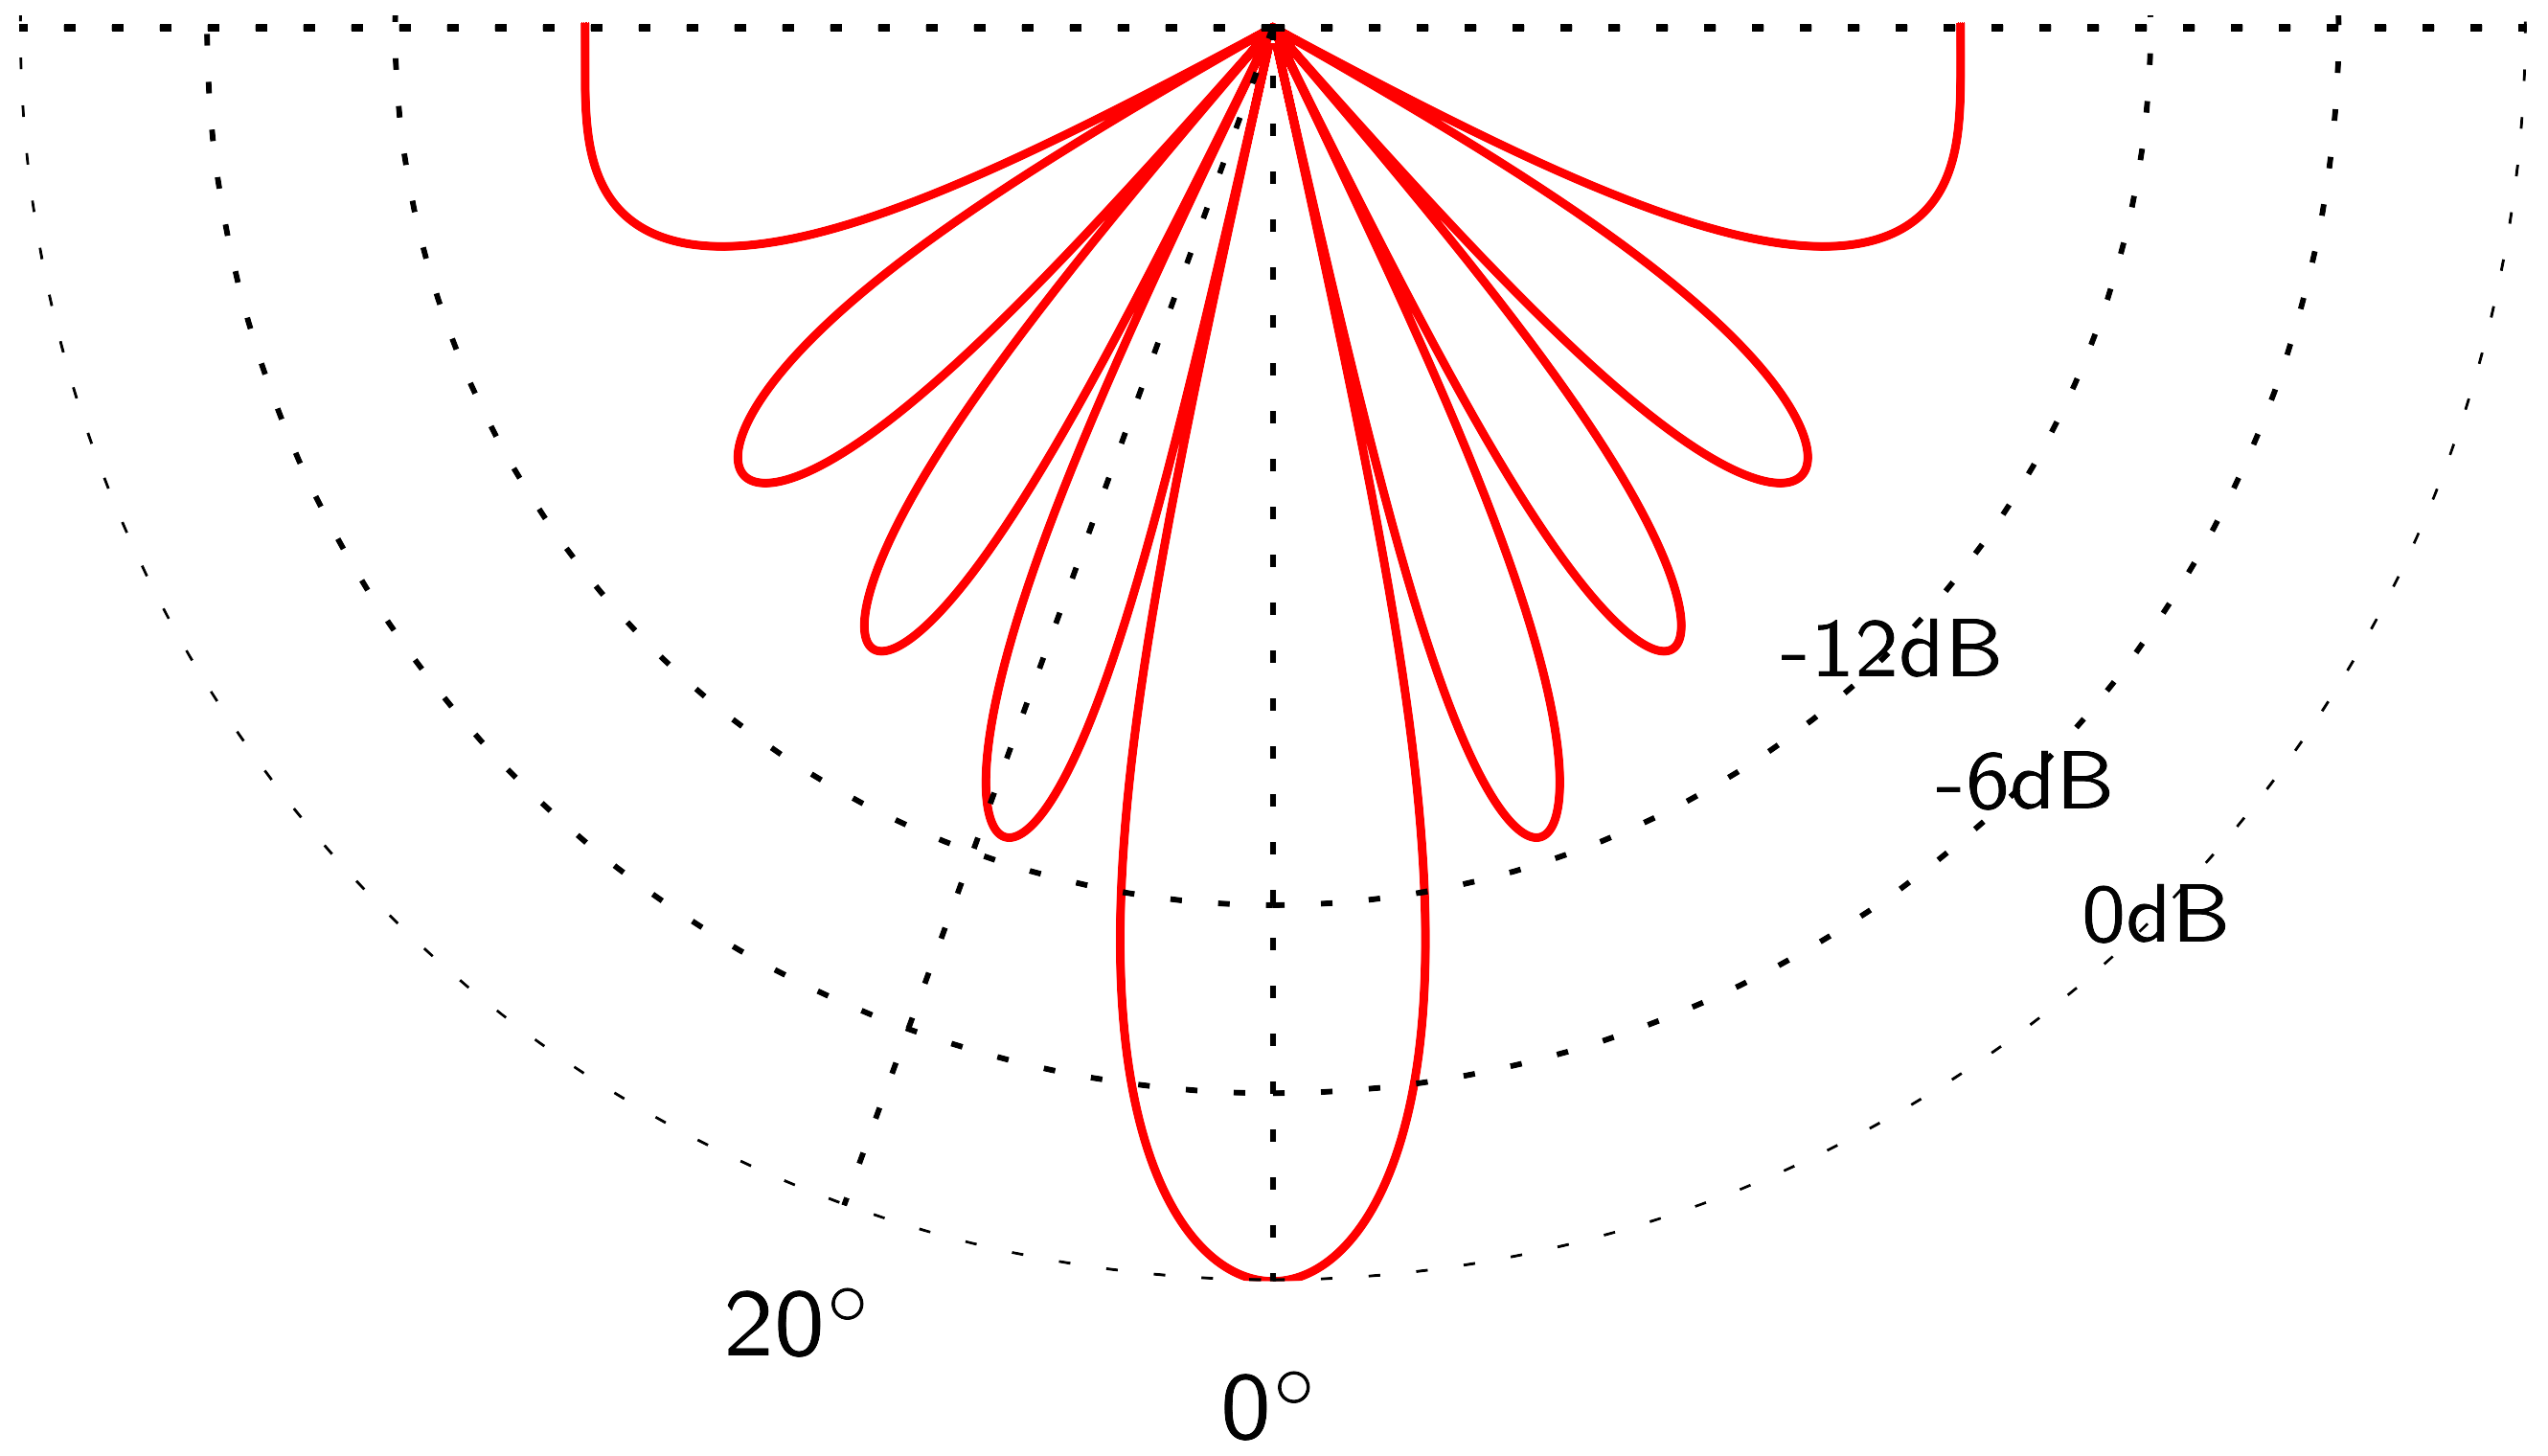
\includegraphics[width=0.47\textwidth]{img/scenario_das_resp2.png}
}
\subfigure[Capon]{
	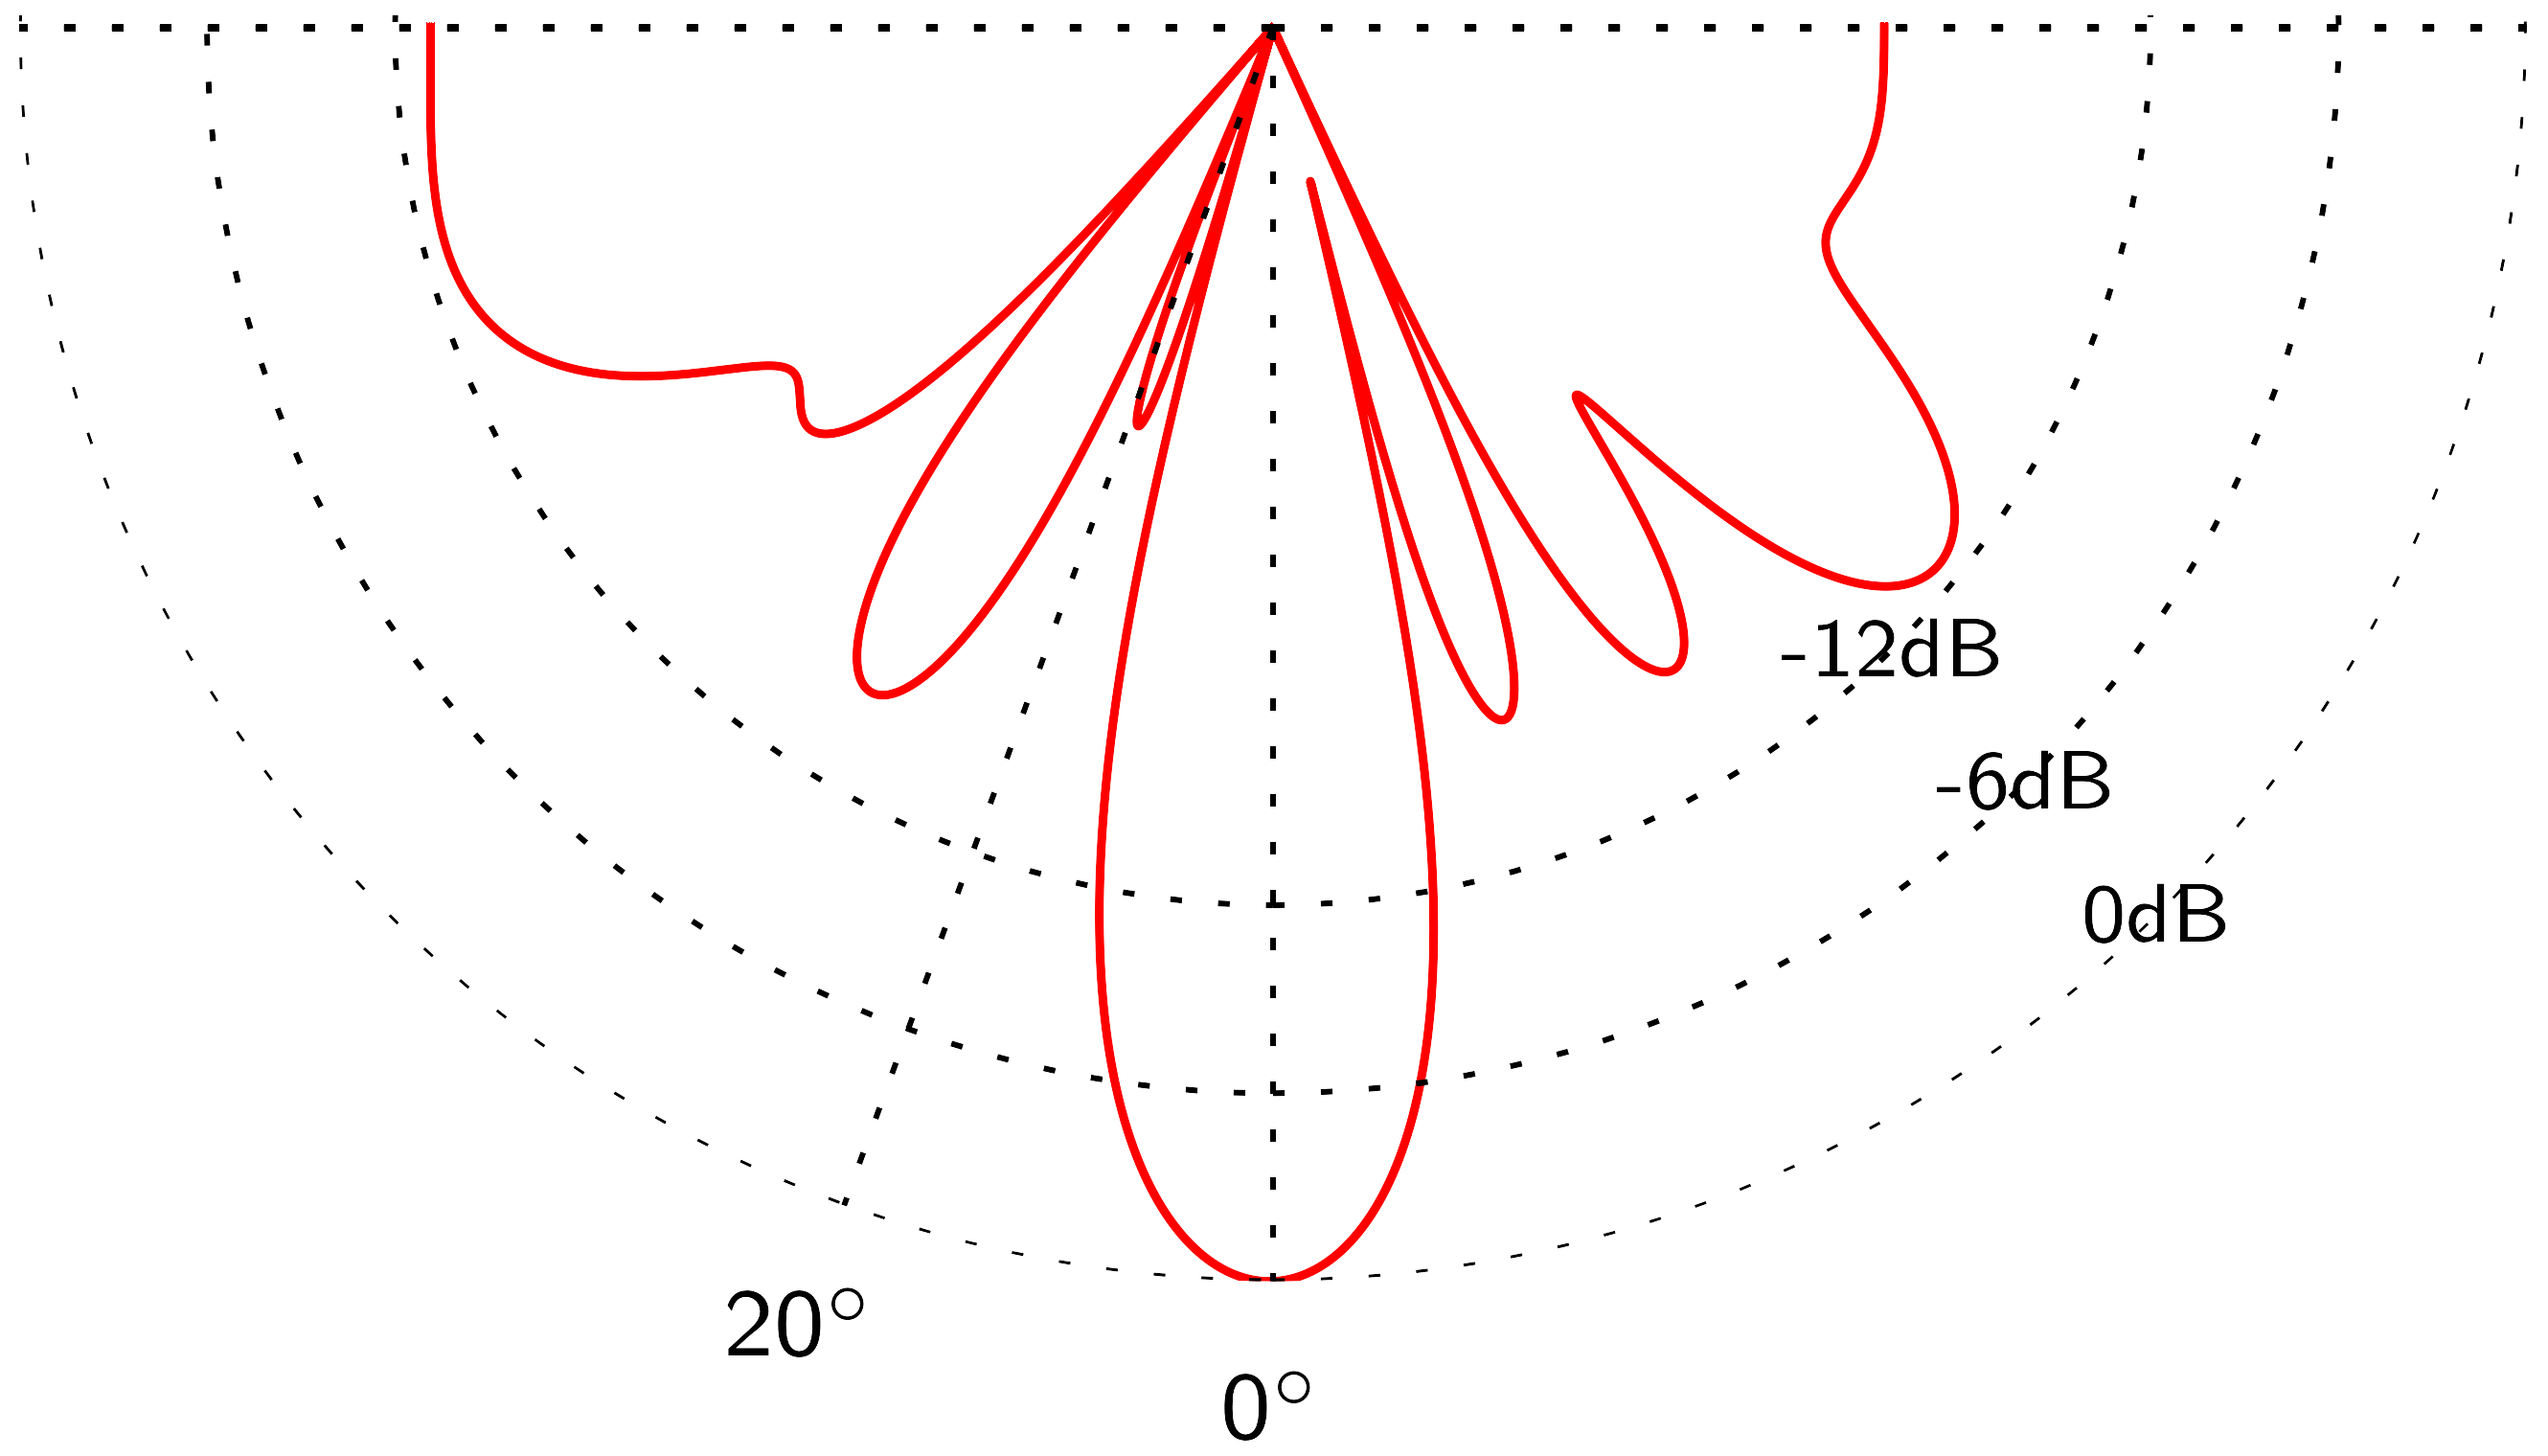
\includegraphics[width=0.47\textwidth]{img/scenario_mv_resp2.png}
}
\caption{Array beam pattern with uniform and Capon weights. An interfering source is located at 20\degree. Notice the reduced sidelobe level for the Capon beam pattern in the direction of the interferer.}
\end{figure}

Capon beamforming\footnote{The name ''Capon beamformer'' is due to work by J. Capon \todo{add citation} on seismic arrays \todo{Move to background.}} or minimum variance beamforming.

Intro to adaptive beamforming. List other variants (LCA, beamspace, Eigen space etc.). 

Beamspace data is typically refers to the polar grid that cardiac ultrasound data is located in prior to scan conversion. In combination with the Capon beamformer, beamspace refers to the K-space representation of the impinging signals (hence the \nom{FFT}{Fast fourier transform} of the channel data). 

Not phase aberration correction.

Add section about the computationally complexity. How many flops are required per rx-beam etc...

Add section about how to present data (max v.s mean etc.)
						
\subsection{Shift invariance}

\section{Volume rendering}\label{sec:volren}

Get section from master theses. Ray casting and opacity functions.

\begin{figure}
\centering
\subfigure[Ray-casting]{
	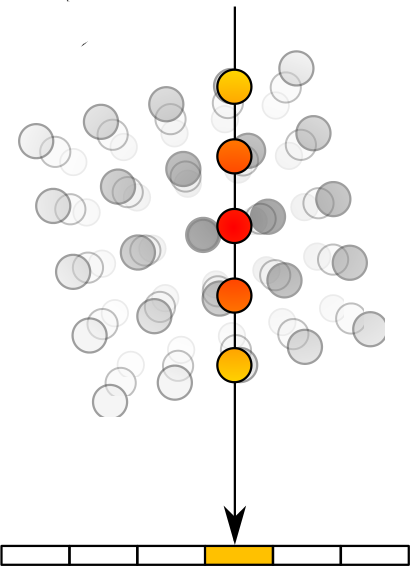
\includegraphics[width=0.4\textwidth]{img/Volumeraycasting.png}
}
\subfigure[Opacity transfer function]{
	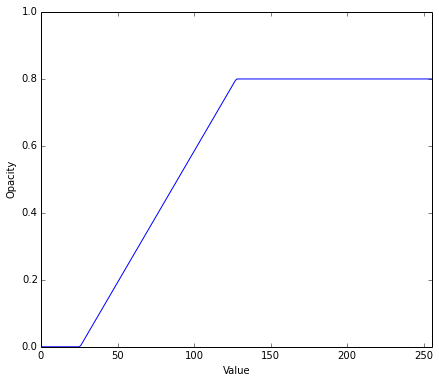
\includegraphics[width=0.5\textwidth]{img/otf.png}
}
\caption{.}
\label{fig:vr}
\end{figure}

\subsection{Adaptive volume rendering}

Visibility driven visualization.

\section{Field simulations}\label{sec:field}

Small chapter about different simulation tools (See hos paper).
			
\endinput
